%\documentclass[twocolumn]{article}
%\usepackage[top=1.2cm, bottom=2cm, right=1cm, left=1cm]{geometry}
%\setlength{\columnsep}{20pt}
\documentclass{article}

\usepackage{hyperref,xcolor}
%\usepackage{algpseudocode}
\usepackage[lined,boxed]{algorithm2e}
\usepackage[english]{babel}
\usepackage{graphicx}
\usepackage{amsmath,amssymb}
\usepackage[utf8x]{inputenc}
\usepackage{graphicx}
\usepackage{subfigure}
\usepackage{dsfont}
\usepackage{url}
\usepackage{hyperref}
\usepackage{geometry}
\usepackage{mathrsfs}
\usepackage[]{mcode}
\usepackage{color}
\usepackage{tikz}
\usetikzlibrary{arrows, decorations.markings}
\usetikzlibrary{shapes.geometric}
\usetikzlibrary{positioning}
\usetikzlibrary{fit}
\usepackage{sidecap}
\usepackage{bbold}
\usepackage{caption}
\usepackage{eurosym}
\usepackage{lipsum}

%\setlength\textwidth{\dimexpr 14cm + 1cm\relax}
%\setlength\columnsep{\dimexpr 1cm\relax}

\definecolor{wine-stain}{rgb}{0,0.4,0.2}
\hypersetup{
  colorlinks,
  linkcolor=wine-stain
}

\definecolor{magenta}{rgb}{1,0,1}
\definecolor{canard}{rgb}{0,1,1}
\definecolor{marron}{rgb}{0.9,0.4,0.1}
\definecolor{marron_noir}{rgb}{0.4,0.1,0}

\DeclareMathOperator*{\argmin}{\arg\!\min}
\DeclareMathOperator*{\argmax}{\arg\!\max}

\geometry{left=3.5cm , right=3cm}
%\geometry{left=1.5cm , right=1cm}

\title{\textbf{\textsc{Algorithmes d'apprentissage pour les chaînes de Markov
cachées}}\vspace{4mm}}
\author{\textbf{Alexis Jacq}\vspace{4mm}}

\begin{document}
%\lipsum
\maketitle

\section{Un peu de philo...}
Pour proposer une explication à un phénomène, dans le but de le prédire ou bien de l'exploiter, l'Homme a recours à des modèles simplifiés de ce phénomène. Ces modèles consistent à projeter le phénomène dans un formalisme accessible afin de le rendre compréhensible et descriptible.  Ainsi, les représentations cognitives du monde qui se forment dans nos cerveaux, nos langages, nos religions et enfin nos modèles scientifiques sont autant de modèles abordés pour s'entendre sur une compréhension -- d'abord personnelle puis commune -- de notre environnement. \\
\\
L'apprentissage consiste à adapter où bien à affiner les modèles choisis afin d'optimiser leur capacité à décrire les phénomènes observés. Toujours dans les mêmes exemples : au niveau du cerveaux, l'apprentissage neuronal nous permet de cerner des concepts toujours plus pertinents et de mémoriser leur dynamique. Au niveau des langages, nous nous efforçons d’acquérir, par les échanges verbaux, un vocabulaire toujours plus adapté à nos sociétés et à nos moeurs, puis l'on suppose ce vocabulaire assez efficace pour l'utiliser et ainsi le tester. Dans les religions, nous cherchons à ``grandir dans la foi", ce qui consiste en un perpétuel effort introspectif d'adaptation aux convictions spirituelles et d'acceptation des idéologies. Enfin, en science, la démarche est plus simple à décrire : établir et supposer des modèles mécanistiques puis affiner leur paramètres pour les adapter à la description du phénomène étudié. L'apprentissage se fait donc en deux étapes : l'\textbf{acceptation} du modèle, puis son \textbf{adaptation}. \\
\\
Ces deux étapes ne sont absolument pas disjointes : en adaptant le modèle d'une certaine façon, on le modifie, et on en accepte un nouveau, etc... L'apprentissage peut donc \^etre vu comme un permanent saute-mouton entre acceptation et adaptation : on accepte le modèle pour établir une prédiction, on adapte le modèle selon l'écart entre ce qui a été prédit et ce qui est advenu, puis on accepte le modèle adapté et on recommence, etc... Il est important de voir que tous les algorithmes ou autres démarches visant un apprentissage reprennent ce schéma d'acceptation/adaptation. 

\section{Un peu de formalisme...}
Nous nous plaçons ici dans le cadre d'un formalisme mathématique. Comme dans la séance précédente \cite{1}, nous nous intéressons à une \textit{classe} de modèles très simples : étant donné le phénomène observé $X\rightarrow Y^{\text{obs}}$ où l'on cherche à expliquer la variable d'intérêt $Y^{\text{obs}}$ avec la variable $X$, on établit le modèle suivant :
\[\mathcal{M}_P:X \mapsto Y\]
\\
où $\mathcal{M}_P$ désigne le modèle (dépendent du jeu de paramètre $P$), vu comme une application qui à $X$ (variable connue) associe $Y$ (la prédiction). Ici, adapter le modèle, c'est optimiser les paramètres $P$ dans le but de minimiser l'erreur de prédiction, à savoir l'``écart" entre $Y$ prédit et $Y^{\text{obs}}$ observé. Comme nous l'avons vu précédemment, la définition de cet écart va beaucoup dépendre du contexte. Dans cette séance, nous allons nous intéresser à un contexte stochastique. La mesure d'erreur de prédiction sera donc définie par la vraisemblance. Cette quantité a déjà été introduite dans la séance précédente (\cite{1} section 2.3.1). Rappelons juste qu'il s'agit de la capacité du modèle à \textit{expliquer} l'observation $Y^{\text{obs}}$. On la note $\mathcal{L}$ (pour \textit{likelihood} = vraisemblance) :
\[\mathcal{L}(\mathcal{M}_P,X,Y^{\text{obs}}) = \mathbb{P}[Y^{\text{obs}}\vert \mathcal{M}_P,X]\]

\section{ ...Maintenant on peut y aller}

Dans cette séance, nous étudions un modèle très particulier : les cha\^ines de Markov cachées (HMM pour Hidden Markov Model). Mais avant tout : qu'est-ce qu'une chaîne de Markov ?

\subsection{Approche non rigoureuse}

Prenons un processus purement aléatoire, par exemple un ``pile ou face". Pourquoi un \textit{processus} ? Parce qu'on va faire plusieurs jetés de suite, ce qui apporte une dimension temporelle. De ce fait, on va pouvoir les nommer par indice, par exemple $j_1$ le premier jeté, $j_2$ le deuxième etc... A chaque fois $j_i$ vaut pile ou face selon le résultat obtenu. Pourquoi \textit{purement} aléatoire ? En fait, un jeté de pièce n'est absolument pas aléatoire : il dépend de la force et du point d'application du coup de pouce, de la position initiale dans l'espace, de la topographie du sol, peut-\^etre m\^eme de la température... Mais à notre échelle, étant incapable d'établir ces liens de causalité, on préfère modéliser le jeté de pièce comme un événement ne dépendant d'absolument rien. Rien ne permet de prédire si le résultat sera pile ou face. \\
\\
Maintenant, regardons un autre processus. On continue à jeter successivement des pièces. Sauf que cette fois-ci, on compte un score. Supposons que l'on joue pile : si le résultat d'un lancer donne pile, on gagne un point, sinon on perd un point. Indiçons l'état de ce score pour étudier son avancement : $s_1$ pour le score après le premier jeté, $s_2$ après le second, etc... Ainsi, $s_n$ représente le score au bout de $n$ jetés :
\[s_1 = \textbf{1}_{[j_1 = \text{pile}]} - \textbf{1}_{[j_1 = \text{face}]}\]
\[s_2 = s_{1} + \textbf{1}_{[j_2 = \text{pile}]} - \textbf{1}_{[j_2 = \text{face}]}\]
\[...\]
\[s_n = s_{n-1} + \textbf{1}_{[j_n = \text{pile}]} - \textbf{1}_{[j_n = \text{face}]}\]
\\
Cette fois-ci, on voit que $s_n$ dépend de $s_{n-1}$ qui est connu à l'instant $n$. En effet si à l'instant $n-1$, le score est à $s_{n-1}=10$ on sait que $s_n$ vaudra 11 ou 9 selon $j_n$. En outre, sans  la connaissance de $s_{n-1}$ on ne pourrait rien prédire de plus que ``$s_n$ sera compris entre -$n$ et +$n$ (inclus) et aura la même parité que $n$". \\
\\
Remarquons autre chose : si on conna\^it $s_{n-1}$, ça ne sert à rien de conna\^itre $s_{n-2}$ pour obtenir des informations à propos de $s_n$. En effet, les informations apportées par $s_{n-2}$ sont incluses dans les informations apportées par $s_{n-1}$. Par ex, si on conna\^it $s_{n-2}=9$ on sait que $s_n$ vaudra 7, 9, ou 11, tandis que si on conna\^it $s_{n-1}=10$, on sait bien que $s_n\in \{7,9,11\}$ mais plus encore : $s_n\in \{9,11\}$. On appelle cela ``propriété d'oubli" ou bien ``propriété de Markov".   C'est dire que si on conna\^ it $s_{n-1}$ et $s_{n-2}$, on peut \textit{oublier} $s_{n-2}$ qui ne sert plus à rien. \\
\\
Plus formellement, on dit que la \textbf{loi} (c'est à dire la nature du modèle stochastique) de $s_n$ \textbf{sachant}  $s_{n-1}$, $s_{n-2}$, ... , $s_2$, $s_1$ est la m\^eme que celle de $s_n$ \textbf{sachant} seulement $s_{n-1}$.\\
\\
Il est très fréquent de rencontrer des modèles stochastiques vérifiant cette propriété. Le premier exemple, et sans doute le plus simple, est celui des \textbf{marches aléatoires}. Il faut imaginer un homme complètement so\^ul errant dans une ville. Tantôt il fait un pas vers la gauche, puis vers l'avant, puis un autre vers la gauche suivit d'un pas en arrière. À chaque instant (les instants ici représentent les pas successifs) la position courante seule donne autant d'information sur la position future que l'intégralité de l'errance depuis la sortie du pub. En fait, les marches aléatoires se généralisent comme des accumulations additives de réalisations d'une variable aléatoire. On peut donc les définir par récurrence  comme suit :
\[z_n = z_{n-1} + x_n\]   
\\
où $z_n$ est la $n$-ème position de la marche, et $x_n$ la $n$-ème réalisation d'une variable aléatoire. Vous l'avez sans do\^ute deviné, le processus défini par les scores de jetés de pièce est donc une marche aléatoire. Mais attention : toutes les cha\^ines de Markov ne sont pas des marches aléatoires ! En effet, on pourrait très bien définir la cha\^ne suivante (cette récurrence s'appelle le \textit{critère fondamental des cha\^ines de Markov}, toute cha\^ine de Markov peut s'écrire sous cette forme et n'importe quelle suite vérifiant cette propriété définie une cha\^ine de Markov): 
\[z_n = \mathit{f}(z_{n-1},x_n,n)\]
\\
où $\mathit{f}$ est mesurable de $\mathbb{R}^2\times\mathbb{N}$ dans $\mathbb{R}$, mais ça (les mesures et tout) on le verra plus loin, si ça vous intéresse. Pour l'instant, nous allons nous contenter de la définition qui est abordée dans le chapitre suivant (je vous rassure, elle est on ne peux plus rigoureuse et suffisante).

\newpage
\subsection{Approche rigoureuse des cha\^ ines de Markov}

Je vais copier-coller (Ha, si seulement on pouvait réellement copier-coller du LateX !) l'introduction aux cha\^ines de Markov du Pr. Jean Jacod que l'on retrouve en début de ses poly de cours à Jussieu (\cite{2},\cite{3}) :\\
\\
\textcolor{marron_noir}{L'idée des cha\^ines de Markov est très simple : il s'agit d'une suite $(X_n)_{n\in \mathbb{N}}$ de variables aléatoires à valeurs dans un espace mesurable $(E,\mathcal{E})$, définies sur un espace de probabilité $(\Omega,\mathcal{F},\mathbb{P})$, et telle que pour tout $n$ on ait la propriété suivante :}\\
\begin{equation}
\textcolor{marron_noir}{\left. \begin{array}{r}
\textcolor{marron_noir}{\text{Conditionnellement à la valeur de $X_n$, les variables $(X_0, ..., X_{n-1})$}}\\
\textcolor{marron_noir}{\text{d'une part, $(X_{n+1},X_{n+1},...)$ d'autre part, sont indépendantes.}}\\
\end{array}\right\rbrace}
\end{equation}
\\
\textcolor{marron_noir}{Ce modèle permet de rendre compte d'un très grand nombre de situations concrètes.}\\
\\
Encore une fois, nous ne nous intéresserons pas pour l'instant à la théorie de la mesure (qui pourrait très bien -- et ce serait une superbe idée -- être la thématique d'un GT à part entière). Donc pour vous expliquer la phrase \textcolor{marron_noir}{...à valeurs dans un espace mesurable $(E,\mathcal{E})$, définies sur un espace de probabilité $(\Omega,\mathcal{F},\mathbb{P})$...}, je vous dirais tout simplement : ``\textit{cela veut dire que tout est bien définie et utilisable dans le contexte voulu}". C'est une phrase qui permet d'écarter tout phénomène pathologique exotique qui pourrait se glisser dans notre définition. Un peu comme une formule de marabou \cite{4} pour repousser les mauvais esprits. \\
\\
Cette définition se réécrit en termes plus symboliques :\\
\\
\textbf{Definition/ Propriété} [\textit{cha\^ine de Markov}] : Soit $(X_n)_{n\in \mathbb{N}}$ une suite de variables aléatoires définies \textit{blablabla} et à valeur dans l'espace mesurable \textit{blablabla}. $(X_n)_{n\in \mathbb{N}}$ définit une cha\^ine de Markov si et seulement si $\forall$ $n$ :

\begin{equation}
\displaystyle \mathbb{P} [ X_{n+1},X_{n+2}, ... \vert X_0, ... X_{n-1}, X_n] = \mathbb{P}[ X_{n+1},X_{n+2}, ... \vert X_n]
\end{equation}
\\
Cette dernière propriété (2) est tout bonnement la \textbf{propriété de Markov faible ``généralisée"} (\textit{faible} car il y a une version forte qui se généralise à un domaine d'application plus étendue \textsf{( elle est super compliquée donc je ne prendrais pas le risque de l'introduire )} et \textit{généralisé} car elle conserne ``tout l'avenir'' sachant ``tout le passé''). Dans ce chapitre, nous ne nous intéressons qu'aux cha\^ines de Markov \textbf{homogènes}. C'est à dire que la loi d'un événement futur $X_{n+1}$ ou de n'importe quelle réunion d’événements futurs $(X_{n+1},X_{n+2}, ...)$ conditionnellement à un événement de départ $X_n$ reste la même quelque soit l'instant $n$. En d'autres termes :\\
\\
\textbf{Propriété} [\textit{homogénéité}] :

\begin{equation}
\displaystyle \forall n,\hspace{3mm}\mathbb{P}[ X_{n+1},X_{n+2}, ... \vert X_n] = \mathbb{P}[ X_{1},X_{2}, ... \vert X_0]
\end{equation}
\\
On établit donc la \textbf{règle d'oubli} des cha\^ines de Markov homogènes :\\
\\
\textbf{propriété} [\textit{règle d'oubli}] :

\begin{equation}
\displaystyle \mathbb{P} [ X_{n+1},X_{n+2}, ... \vert X_0, ... X_{n-1}, X_n] = \mathbb{P}[ X_{1},X_{2}, ... \vert X_0]
\end{equation}
\\
Cette dernière propriété sera très importante par la suite. Notons que l'homogénéité peut aussi se voir comme la simplification du critère fondamental : $(Z_n)_{n\in\mathbb{N}}$ est une cha\^ ine de Markov homogène si et seulement si ses réalisations $(z_n)_{n\in\mathbb{N}}$ vérifient la récurrence suivante :
\[z_n = \mathit{f}(z_{n-1},x_n)\]
\\
où $\mathit{f}$ est mesurable de $\mathbb{R}^2$ dans $\mathbb{R}$ et les $(x_n)_{n\in\mathbb{N}}$ sont les réalisations d'une suite de variables aléatoires $(X_n)_{n\in\mathbb{N}}$ toutes de même loi et telles que toutes les combinaisons possibles $(X_n)_{n\in\mathbb{I}\subset\mathbb{N}}$ soient indépendantes de $Z_0$.


\subsection{Cha\^ines de Markov cachées}

Voilà, normalement on ne devrait pas avoir besoin de plus de notions que ça pour aborder les HMM. Pour ceux qui veulent approfondir les outils et ustensiles des cha\^ines de Markov, je conseillerai le poly du GT de François Bienvenu sur les modèles matriciels de populations \cite{5} (ou bien, évidement, un vrai bouquin de votre BU, mais çe sera probablement super sérieux et ennuyeux alors que nos notes à nous sont vraiment cool). Nous pouvons maintenant nous poser la question qui nous démangeait tant : \textit{Mais où se cachent donc les chaînes de Markov cachées} ?\\
\\
Bon, posons-nous une question un peu plus fine : Qu'est-ce qu'une chaîne de Markov \textit{cachée} ? C'est avant tout un modèle. Et la meilleur façon d'introduire un modèle, c'est de présenter un phénomène très simple qui se modélise très bien avec. Je ne ferais pas la même erreur que celle de mon professeur de première année de master qui était allé chercher la probabilité d'apparition des îlots CpG à proximité des promoteurs dans l'ADN. Ce phénomène d'apparition de ces îlots non-méthylés est très intéressant à modéliser avec des chaînes de Markov cachées mais bon... Il y a vraiment plus simple comme intro...\\
\\
Prenons deux mecs bourrés à la sortie d'un bar. Nous allons faire la supposition suivante : l'un (Pierrot) est vraiment foutu et entame donc une marche aléatoire. L'autre (Robert) a un peu moins bu : il essaye comme il le peut de suivre Pierrot pour ne pas le perdre de vue. Mais bon, il en a quand même un bon coup dans le nez et les choses sont moins simples qu'elles en ont l'air : il n'y voit plus rien. Pierrot-aléatoire se sent rassuré de la présence bienveillante de son ami Robert qui essaye de le suivre. Mais il ne peut pas s'arrêter de marcher et a beaucoup de mal à contrôler ses jambes. Lorsqu'il s'écarte de son ami, il pousse un cri de détresse ``HAAAAOOOO". Quand il s'en rapproche, il pousse un cri rassuré ``HOOOOOOO". Robert utilise ces cris pour le repérer et le suivre. \\
\\
Le problème est le suivant : Pierrot pousse des cris approximatifs et se trompe parfois. \\
\\
\underline{Formalisons cette situation :} Il y a deux ``états" possibles pour Pierrot : soit il se rapproche (état $x_1$), soit il s'écarte (état $x_2$). Notons $X_n$ la variable aléatoire qui représente l'état dans lequel se trouve Pierrot à l'instant $n$. Lorsque Pierrot prend une direction, il a du mal à s'en défaire tout de suite. Je veux dire par là que lorsqu'il commence à s'écarter, il essaye de se sortir de cette situation mais c'est difficile. Disons qu'il a, à chaque instant $n$ où il s'écarte, une probabilité de revenir vers Robert $\mathbb{P}[X_{n+1} = x_1 \vert X_n=x_2] = 0.4$ ; Bien entendu cela implique $\mathbb{P}[X_{n+1} = x_2 \vert X_n=x2] = 0.6$ pour la probabilité de continuer à s'écarter. D'autre part, si Pierrot sent qu'il se rapproche, il fait attention à ne pas perdre ce bon plie. Sa probabilité de rester dans cet état de rapprochement est donc élevée $\mathbb{P}[X_{n+1} = x_1 \vert X_n=x_1] = 0.7$ ; ce qui implique $\mathbb{P}[X_{n+1} = x_2 \vert X_n=x_1] = 0.3$. Comme Pierrot est sacrément bourré, à chaque instant il oublie le passé. Bref, $\mathbb{P}[X_{n+1} \vert X_n, X_{n-1} ... X_0] = \mathbb{P}[X_{1} \vert X_0]$. On est clairement face à une chaîne de Markov à deux états. Plus haut, j'ai parlé de marche aléatoire : il s'agissait de chaînes de Markov à nombre infini d'états (la variable aléatoire représentant l'état à l'instant $n$ de la chaîne que je notais $Z_n$ pouvait prendre n'importe quelle valeur entière entre $-\infty$ et $+\infty$ selon la grandeur de $n$ alors qu'ici notre variable $X_n$ de la chaîne-Pierrot prend comme valeur $x_1$ ou bien $x_2$ quelque soit $n$). \\
\\
Dans une HMM, les probablilités liées à la chaîne décrivent ce qu'on appelle les
\textbf{lois de transition} : elles régissent le passage d'un état à l'autre. \\
\\
Pour ce qui est des cris que pousse Pierrot, écrivons qu'il y a deux cris  possibles : $o_1$ (HOOOOO) et $o_2$ (HAAAOO). Notons aussi $O_n$ la variable aléatoire qui représente le cri poussé à l'instant $n$. Nous utilisons des $\mathcal{O}$ parce qu'il s'agit d'$\mathcal{O}$bservations. Disons donc que la probabilité que Pierrot pousse le bon cri quand il est dans l'état de rapprochement $x_1$ est $\mathbb{P}[O_{n+1} = o_1 \vert X_n=x_1] = 0.8$ et que la probabilité qu'il pousse le bon cri quand il s'écarte ($x_2$) est $\mathbb{P}[O_{n+1} = o_2 \vert X_n=x_2] = 0.7$. Ces probabilité sont appelées \textbf{lois d'émission}. Dans notre exemple, il n'y a que deux cris possibles : $\mathbb{P}[O_{n+1} = o_2 \vert X_n=x_1] = 0.2$ et $\mathbb{P}[O_{n+1} = o_1 \vert X_n=x_2] = 0.3$. \\
\\
La manière la plus simple de représenter graphiquement ce processus est de dessiner un ``peigne'' : le temps s'écoule de gauche à droite et de l'instant $n$ à l'instant $n+1$ on passe de l'état $X_n$ à l'état $X_{n+1}$. À chaque instant, un signal observable (cri) est émis (verticalement). Sur le graphe suivant, les états sont representés par des carrés, et les signaux observables par des ronds :
\\
\begin{center}

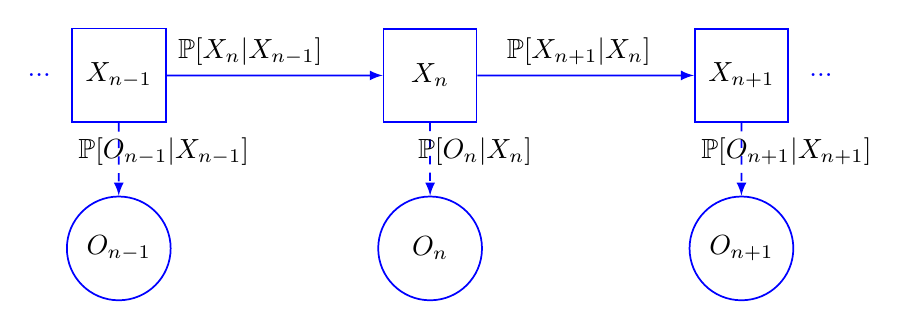
\begin{tikzpicture}
[every node/.style={inner sep=0pt}]
\node (1) [regular polygon, regular polygon sides=4, minimum size=37.5pt, fill=white, line width=0.625pt, draw=blue] at (100.0pt, -87.5pt) {\textcolor{black}{$X_{n-1}$}};
\node (2) [regular polygon, regular polygon sides=4, minimum size=47.5pt, fill=white, line width=0.625pt, draw=blue] at (212.5pt, -87.5pt) {\textcolor{black}{$X_{n}$}};
\node (3) [regular polygon, regular polygon sides=4, minimum size=37.5pt, fill=white, line width=0.625pt, draw=blue] at (325.0pt, -87.5pt) {\textcolor{black}{$X_{n+1}$}};
\node (4) [circle, minimum size=37.5pt, fill=white, line width=0.625pt, draw=blue] at (212.5pt, -150.0pt) {\textcolor{black}{$O_{n}$}};
\node (5) [circle, minimum size=37.5pt, fill=white, line width=0.625pt, draw=blue] at (325.0pt, -150.0pt) {\textcolor{black}{$O_{n+1}$}};
\node (6) [circle, minimum size=37.5pt, fill=white, line width=0.625pt, draw=blue] at (100.0pt, -150.0pt) {\textcolor{black}{$O_{n-1}$}};
\draw [line width=0.625, ->, >=latex, color=blue] (2) to  (3);
\draw [line width=0.625, ->, >=latex, dashed, color=blue] (2) to  (4);
\draw [line width=0.625, ->, >=latex, dashed, color=blue] (3) to  (5);
\draw [line width=0.625, ->, >=latex, color=blue] (1) to  (2);
\draw [line width=0.625, ->, >=latex, dashed, color=blue] (1) to  (6);
\node at (266.25pt, -78.75pt) {\textcolor{black}{$\mathbb{P}[X_{n+1}\vert X_{n}]$}};
\node at (228.75pt, -115.pt) {\textcolor{black}{$\mathbb{P}[O_{n}\vert X_{n}]$}};
\node at (341.25pt, -115.pt) {\textcolor{black}{$\mathbb{P}[O_{n+1}\vert X_{n+1}]$}};
\node at (147.5pt, -78.75pt) {\textcolor{black}{$\mathbb{P}[X_{n}\vert X_{n-1}]$}};
\node at (116.25pt, -115.pt) {\textcolor{black}{$\mathbb{P}[O_{n-1}\vert X_{n-1}]$}};
\node at (353.75pt, -87.5pt) {\textcolor{blue}{...}};
\node at (71.25pt, -87.5pt) {\textcolor{blue}{...}};
\end{tikzpicture}

\end{center}

Intéressons-nous maintenant à quelques petites propriétés qui découlent d'une telle structure...

\subsubsection{Quelques propriétés qui découlent de cette structure}
%loi de la serie des etats
%loi de la serie des observation
%forward-backward etc

\subsection{L'algorithme EM}

Comme nous l'avons fait remarqué dans notre introduction, l'apprentissage de manière général peut être vu comme une répétition d'étapes d'acceptation et d'adaptation. Nous allons voir que c'est exactement le principe de l'algorithme EM. Mais déjà : que veut dire ``EM" ? C'est pour Expectation-Maximisation. Car effectivement, c'est un algorithme qui répète en boucle deux étapes de calcul. La première évalue l'espérance de la vraisemblance du modèle en acceptant des paramètres, et la deuxième adapte les paramètres de manière à maximiser cette espérence, et ainsi de suite...\\
\\
Ok, tout ça est bien dit mais ça manque gravement de clarté. D'abord, ne nous perdons pas : \textbf{l'algorithme EM est un algorithme de Clusturing}. Quelle rapport avec les HMM ? Nous allons voir ça plus loin. Mais j'insiste sur ce point pour dire que ici, nous regardons un ensemble de \textbf{N sacs}, et de \textbf{M billes}. Chaque bille appartient à un sac. Notre modèle, c'est l'ensemble des assignations bille-sac. Si maintenant, chaque bille a une probabilité d'appartenir à un sac, alors le modèle que l'on cherche sera l'ensemble des assignations bille-sac qui maximisent ces probabilités. 

\subsection{L'agorithme de Viterbi}
\newpage
\begin{thebibliography}{9}

\bibitem{1}
  Jacq, A., Bienvenu, F. (2013)
  \emph{Introduction à l'apprentissage}.
  séance GT n.8
  
\bibitem{2}
  Jacod, J. (2003)
  \emph{Cha\^ines de Markov, Processus de Poisson et Applications}.
  Poly. de cours
  
\bibitem{3}
  Jacod, J. (2004)
  \emph{Processus de Markov, application à la dynamique des populations}.
  Poly. de cours

\bibitem{4}
  Metalshine (2047)
  \emph{Les distances n'existent pas}.
  
\bibitem{5}
  Bienvenu, F. (2013)
  \emph{Introduction aux modèles matriciels de populations}.
  séance GT n.6,7
  
  
\end{thebibliography}

\end{document}

